\documentclass[floatfix,nofootinbib,superscriptaddress,fleqn]{revtex4-2} 
%\documentclass[aps,epsfig,tightlines,fleqn]{revtex4}
\usepackage[utf]{kotex}
\usepackage[HWP]{dhucs-interword}
\usepackage[dvips]{color}
\usepackage{graphicx}
\usepackage{bm}
%\usepackage{fancyhdr}
%\usepackage{dcolumn}
\usepackage{defcolor}
\usepackage{amsmath}
\usepackage{amsfonts}
\usepackage{amssymb}
\usepackage{amscd}
\usepackage{amsthm}
\usepackage[utf8]{inputenc}
 \usepackage{setspace}
 \usepackage{tikz}
%\pagestyle{fancy}

\begin{document}

\title{\Large 2022년 1학기 물리학 I: Quiz 12}
\author{김현철\footnote{Office: 5S-436D (면담시간 매주
    화요일-16:00$\sim$20:00)}} 
\email{hchkim@inha.ac.kr}
\author{Lee Hui-Jae} 
\email{hjlee6674@inha.edu}
\affiliation{Hadron Theory Group, Department of Physics,
Inha University, Incheon 22212, Republic of Korea }
\date{Spring semester, 2022}

\vspace{1.cm}

\maketitle


\noindent {\bf 문제 1. (20 pt)}
아래 그림과 같이 끈의 길이가 $l$로 같은 두 진자의 끝에 질량이 각각
$m$, $M$인 두 공이 달려 있다. 질량이 $m$인 공을 $d$만큼 높은 위치까지 
들어올렸다가 놓았다. 여기서 끈의 질량은 무시한다. 완전 비 탄성충돌이
일어나는 경우 충돌 직후에 합쳐진 물체의 속력은 얼마인가? 
\begin{figure}[ht]
  \centering
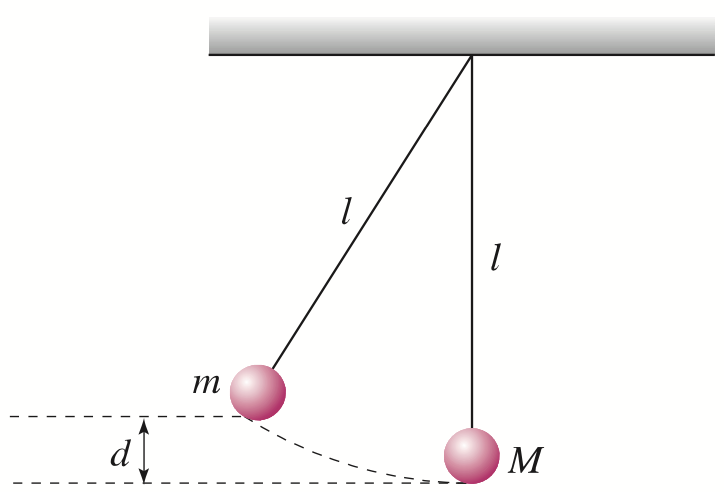
\includegraphics[scale=0.5]{Qfig12-1-20210409.png}
  \caption{문제 1}
  \label{fig:1}
\end{figure}


\noindent {\bf 풀이 : }
맨처음 두 진자가 가지고 있는 역학적 에너지의 합을 $E_i$라 하자. $E_i$는,
\begin{align}
  E_i = mgd.
\end{align}
질량이 $M$인 진자는 충돌 직전까지 정지해 있었으므로 충돌 직전 $E_i$는 
모두 질량이 $m$인 진자의 운동에너지로 전환되었다. 충돌 직전 질량이 $m$인
진자의 속력을 $v_0$라고 하면,
\begin{align}
  v_0 = \sqrt{\frac{2E_i}{m}} = \sqrt{2gd}.
\end{align}
두 진자는 완전 비탄성 충돌을 한다. 충돌 직후 두 진자의 속력을 $v_1$이라 하면,
\begin{align}
  mv_0 = (m+M)v_1,\,\,\,v_1 = \frac{m}{m+M}v_0.
\end{align}
따라서 충돌 직후 합쳐진 물체의 속력 $v_1$은 다음과 같다.
\begin{align}
  v_1 = \frac{m\sqrt{2gd}}{m+M}.
\end{align}
\vspace{1.cm}

\noindent {\bf 문제 2. (40 pt)}
다음 그림과 같이 길이가 $L$인 기차의 왼쪽 벽($x=0$)에 질량이 $m$인 
철수가 서 있다. 철수와 기차는 모두 정지해 있다. 이제, 철수가 기차의
오른쪽 벽으로 이동한다. 기차의 질량이 $M$이고 기차와 선로 사이에는
마찰이 없다. 
\begin{figure}[htp]
  \centering
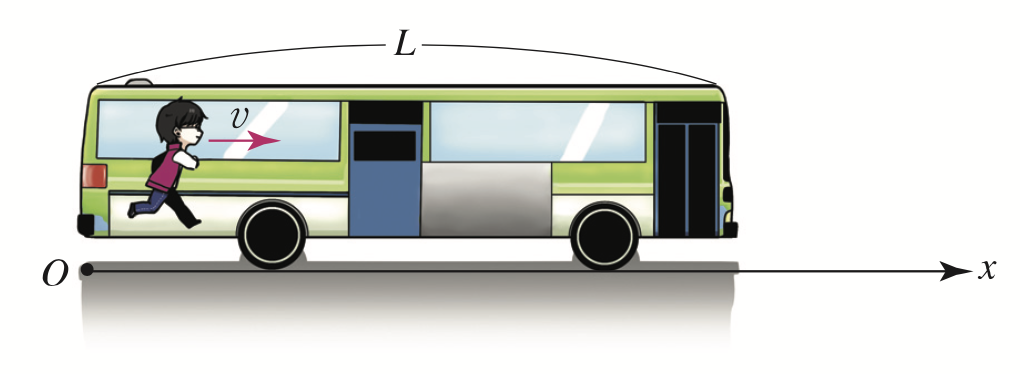
\includegraphics[scale=0.5]{Qfig12-2-20210409.png}  
  \caption{문제 2}
  \label{fig:2}
\end{figure}

\begin{itemize}
\item[(가)] 철수가 기차의 왼쪽 벽에 서 있을 때(즉 철수의 위치가
  $x=0$일 때) 기차와 철수를 합한 전체 계의 질량중심의 좌표
  $x_{\mathrm{cm}}$ 을 구하여라. 
\item[(나)] 초기에 정지해 있던 철수가 속력 $v$로 움직일 때 기차와
  철수를 합한 전체의 선운동량은 얼마인가? (단, 이 경우 철수의 속력
  $v$는 외부에 정지한 관측자가 본 속력이다.) 
\item[(다)] 철수가 속력 $v$로 움직이는 동안 기차가 움직이는 속력은
  얼마인가? 
\item[(라)] 철수가 기차의 오른쪽 벽까지 갔을 때 기차와 철수를 합한
  전체의 질량중심의 좌표는 얼마이어야 하는가?
\item[(마)] 철수가 이동하는 동안 기차도 움직였다면, 철수가 기차의
  오른쪽 벽까지 갔을 때 기차가 움직인 거리는 얼마인가?
\end{itemize}

\noindent {\bf 풀이 : }
\begin{itemize}
\item[(가)] 철수는 $x=0$에 위치해 있으므로 철수의 질량중심은 0이다.
기차의 질량중심을 $x_t$라고 하자. 기차의 질량이 균일하게 분포해있다고 하면,
\begin{align}
  x_t = \frac{1}{M}\int r\,dm = \frac{1}{M}\int_0^L r\rho\,dr .
\end{align}
기차의 밀도 $\rho$는 질량에 길이를 나눈 것이므로,
\begin{align}
  x_t = \frac{1}{M}\int_0^L\frac{M}{L}r\,dr = \frac{1}{2}L.
\end{align} 
따라서 전체 질량중심 $x_{cm}$은 다음과 같다.
\begin{align}\label{eq:1-1}
  x_{cm} = \frac{0+Mx_t}{m+M} = \frac{ML}{2(m+M)}.
\end{align}
\item[(나)] 계의 총 선운동량은 외력에 의존한다. 철수가 $v$로 움직일 때 전체 계에
외력이 작용하지 않으므로 전체의 선운동량은 변하지 않는다. 처음에 철수와 기차 모두 정지해
있었으므로 전체의 선운동량은 0이다. 
\item[(다)] 총 선운동량이 0이므로 철수의 운동량과 기차의 운동량의 합은 0이다. 기차의 속력을 
$v_t$라고 하면 기차와 철수의 운동 방향이 반대이므로,
\begin{align}
  mv + (-Mv_t) = 0,\,\,\, v_t = \frac{m}{M}v.
\end{align}
이다.
\item[(라)] 전체의 선운동량이 변하지 않으므로 전체의 질량중심 또한 변하지 않는다. 철수가 
오른쪽 벽까지 갔을때 전체의 질량중심의 좌표는,
\begin{align}
  x_{cm} = \frac{ML}{2(m+M)}.
\end{align}
이다.
\item[(마)] 기차가 거리 $d$만큼 움직였다고 하자. 
전체의 질량중심은 변하지 않고 철수가 $x=L-d$에 위치하므로 
이 때 기차의 질량중심의 좌표 $x_{t2}$는,
\begin{align}
  x_{t2} = \frac{L}{2}-d. 
\end{align}
식 (\ref{eq:1-1})에 의해,
\begin{align}
  x_{cm} = \frac{ML}{2(m+M)}=\frac{m(L-d)+Mx_{t2}}{m+M}
  =\frac{1}{m+M}\left(m(L-d)+M\left(\frac{L}{2}-d\right)\right) .
\end{align}
따라서 기차가 움직인 거리 $ d$는,
\begin{align}
  \begin{split}
    \frac{1}{2}ML = mL+\frac{1}{2}ML -(m+M)d,\,\,\,
    d=\frac{mL}{m+M},
  \end{split}
\end{align}
이다.
\end{itemize}

\vspace{1.cm}

\noindent {\bf 문제 3. (30pt)}
그림~\ref{fig:3}에서처럼 질량 $m_1$인 물체 1이 정지상태에서 출발한 뒤,
마찰이 없는 비탈을 따라 높이 $h=2.50\,\mathrm{m}$를 미끄러져 내려와 
질량 $m_2=2.00m_1$인 정지해 있는 물체 2와 충돌하였다. 충돌 뒤, 물체
2는 운몽마찰계수가 $\mu_k=0.500$인 영역으로 들어와서 거리 $d$만큼
가다가 멈췄다. 
\begin{figure}[ht]
  \centering
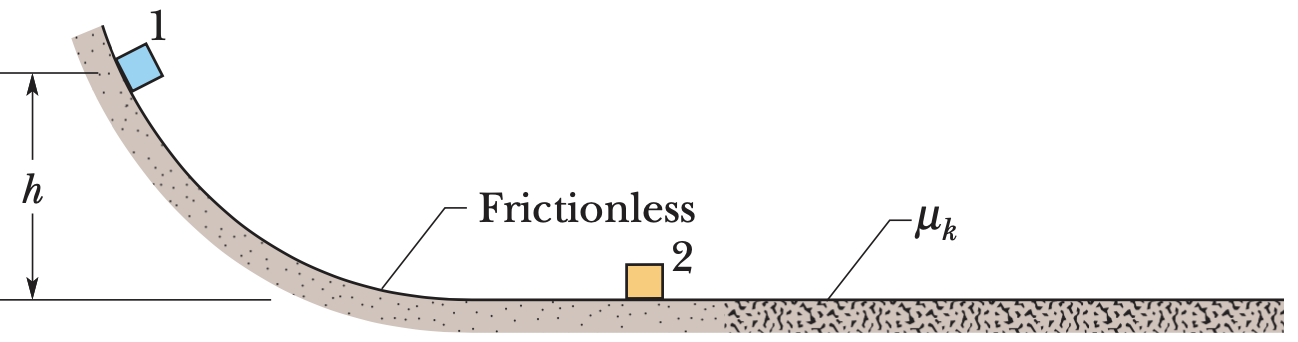
\includegraphics[scale=0.5]{Qfig12-3-20210409.png}
  \caption{문제 3}
  \label{fig:3}
\end{figure}
\begin{itemize}
\item[(가)] 탄성출동일 때와
\item[(나)]  비탄성충돌일 때 $d$는 각각 얼마인가? 
\end{itemize}

\noindent {\bf 풀이 : }
\begin{itemize}
  \item[(가)] 처음 역학적 에너지를 $E_i$라고 하면 $E_i$는 물체 1이 가진 위치에너지 뿐이므로,
  \begin{align}
    E_i = m_1gh.
  \end{align} 
  $E_i$는 충돌 직전 시점에 물체 1의 운동에너지로 전환되었다. 충돌 직전 물체 1의 속력을 $v$라고
  하면,
  \begin{align}\label{eq:2-1}
  \frac{1}{2}m_1v = E_i = m_1gh,\,\,\, v = \sqrt{2gh}.  
  \end{align} 
  두 물체가 탄성충돌 하므로 충돌 이후
  물체 1의 속도를 $v_1$, $v_2$라고 하면,
  \begin{align}
    \begin{split}
      &m_1v = m_1 v_1 + m_2 v_2  \\
      &\frac{1}{2}m_1v^2=\frac{1}{2}m_1v_1^2+\frac{1}{2}m_2v_2^2.
    \end{split}
  \end{align}
  식 \eqref{eq:2-1}에 의해,
  \begin{align}
      \label{eq:2-2}&m_1\sqrt{2gh} = m_1 v_1 + m_2 v_2  \\
      \label{eq:2-3}&m_1gh=\frac{1}{2}m_1v_1^2+\frac{1}{2}m_2v_2^2.
  \end{align}
  식 \eqref{eq:2-2}에 의해,
  \begin{align}\label{eq:2-4}
    m_2v_2 = m_1(\sqrt{2gh}-v_1),
  \end{align}
  이고, 식 \eqref{eq:2-3}에 2를 곱하고 식 \eqref{eq:2-4}를 대입하면,
  \begin{align}
    \begin{split}
      2m_1gh = m_1v_1^2+m_1(\sqrt{2gh}-v_1)v_2.
    \end{split}
  \end{align}
  우변의 첫 항을 좌변으로 옮기고 인수분해하면 다음과 같다.
  \begin{align}
    m_1(\sqrt{2gh}+v_1)(\sqrt{2gh}-v_1) = m_1(\sqrt{2gh}-v_1)v_2.
  \end{align}
  따라서,
  \begin{align}
    v_2 = \sqrt{2gh} + v_1.
  \end{align}
  $v_2$를 다시 \eqref{eq:2-2}에 대입하여 다음을 얻을 수 있다.
  \begin{align}
    m_1\sqrt{2gh} = m_2\sqrt{2gh}+ (m_1 + m_2)v_1,\,\,\,
    v_1 =   \frac{\sqrt{2gh}(m_1-m_2)}{m_1+m_2}.
  \end{align}
  따라서 $v_2$는,
  \begin{align}\label{eq:2-5}
    v_2 = \frac{2m_1\sqrt{2gh}}{m_1+m_2}.
  \end{align}
  물체 2가 마찰력인 존재하는 영역에서 운동하면 마찰력에 의해 운동에너지를 잃고 정지한다.
  물체 2에 작용하는 마찰력 $f_k$와 마찰력이 물체 2가 멈출 때 까지 한 일 $W_k$는,
  \begin{align}
    f_k = \mu_kN = \mu_km_2g,\,\,\,W_k = -f_kd=-\mu_km_2gd.
  \end{align}
  마찰력과 물체가 움직이는 방향이 반대이기 때문에, $W_k$의 부호는 $-$이다. 
  마찰력이 물체 2에 한 일은 물체 2의 운동에너지 변화량과 같다. 즉,
  \begin{align}
  W_k = -\mu_km_2gd = \Delta E_k  
  = 0 - \frac{1}{2}m_2v_2^2 = - \frac{1}{2}m_2v_2^2
  ,\,\,\,d=\frac{v_2^2}{2\mu_k g}.
  \end{align}
  식 \eqref{eq:2-5}에 의해,
  \begin{align}
    \begin{split}
      d&=\frac{4m_1^2h}{(m_1+m_2)^2\mu_k}
      =\frac{4m_1^2(2.50\,\mathrm{m})}{(3.00\,m_1)^2(0.500)}   \\
       &=\frac{4(2.50\,\mathrm{m})}{9.00(0.500)}  \\
       &=2.22\,\mathrm{m}.
    \end{split}
  \end{align}
  탄성충돌한 물체 2는 $2.22\,\mathrm{m}$만큼 움직인다.
  \item[(나)] 공이 완전 비탄성충돌한다고 하자. 충돌 후 속력을 $v_0$라고 하면
   식 \eqref{eq:2-2}으로 부터,
  \begin{align}
    m_1\sqrt{2gh} = (m_1 + m_2) v_0.
  \end{align}
  따라서 $v_0$는,
  \begin{align}
    v_0 = \frac{m_1\sqrt{2gh}}{m_1 + m_2}.
  \end{align}
  완전 비탄성충돌한 물체에 작용하는 마찰력 $f_k$와 마찰력이 물체가 멈출 때 까지 
  한 일 $W_k$는,
  \begin{align}
    f_k = \mu_k N = \mu_k(m_1+m_2),\,\,\,W_k = -f_kd=-\mu_k(m_1+m_2)gd.
  \end{align}
  $W_k$는 물체의 운동에너지 변화량과 같다. 따라서,
  \begin{align}
    -\mu_k(m_1+m_2)gd = \Delta E_k 
    = 0-\frac{1}{2}(m_1+m_2)v^2_0 = -\frac{1}{2}(m_1+m_2)
    \left( \frac{m_1\sqrt{2gh}}{m_1 + m_2} \right)^2.
  \end{align}
  양변을 $(m_1+m_2)$로 나누고 $d$에 대해 정리하면,
  \begin{align}
    \begin{split}
      d &= \frac{m_1^2h}{(m_1+m_2)^2\mu_k} 
        = \frac{m_1^2(2.50\,\mathrm{m})}{(3.00m_1)^2(0.500)}  \\
      &= 0.556\,\mathrm{m}.
    \end{split}
  \end{align}
  완전 비탄성충돌한 물체는 $0.556\,\mathrm{m}$만큼 움직인다.
  \end{itemize}


\vspace{1.cm}

\noindent {\bf 문제 4. (40pt)}
질량 $m$, 반지름 $r$ ($r\ll R)$인 공이 그림~\ref{fig:4}과 같이
미끄러지지 않고 굴러내려오고 있다. 이 공이 반지름 $R$인 원형경로
밑바닥에서부터 높이 $h$인 위치에 공의 가장 낮은 지점이 닿아있다. 공을
정지상태에서 놓으면
\begin{figure}[htp]
  \centering
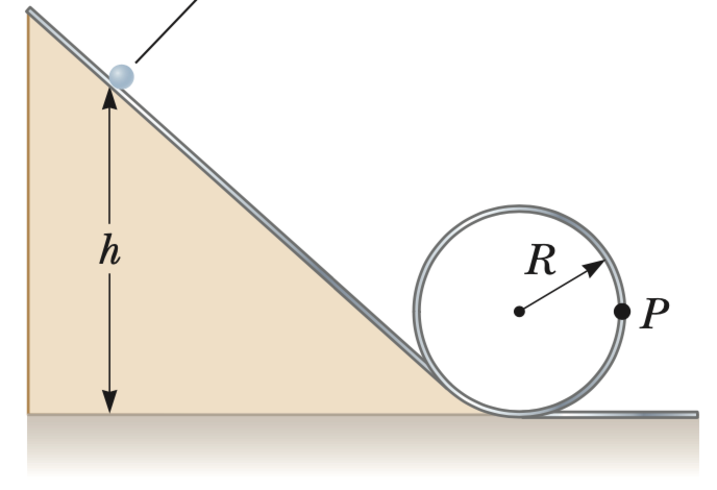
\includegraphics[scale=0.6]{Qfig12-1.pdf}  
  \caption{문제 4}
  \label{fig:4}
\end{figure}
\begin{itemize}
\item[(가)] 공이 원형궤도를 완전히 한바퀴돌 수 있는 $h$의 최소값은
  얼마인가? $r$과 $R$로 표현하여라.
\item[(나)] $h=3R$이면, $P$점에서 공에 작용하는 힘의 성분들은
  얼마인가?   
\end{itemize}

\noindent {\bf 풀이 : }
\begin{itemize}
  \item[(가)] 처음 공이 가지고 있는 역학적 에너지 $E_i$는 다음과 같다.
  \begin{align}
    E_i = mg(h+r).
  \end{align}
  공이 원형궤도를 완전히 한바퀴 돌기 위해 원형궤도의 꼭대기 지점에서 속력이 충분히
  커야한다. 꼭대기 지점에서 공의 자유 물체 다이어그램을 그려보면 다음과 같다.

  \begin{figure}[htp]
    \centering
    \begin{tikzpicture}
      \draw (0,-1.5) -- (0,1.5) ;
      \draw (-1.5,0) -- (1.5,0) ;
      \draw [red,very thick,-latex] (0,-0.1) -- (0,-1.4) 
      node [left,black] {$F_g$};
      \draw [red,very thick,-latex] (0,-0.1) -- (0,-0.8) 
      node [right,black] {$N$};
      \draw [blue,very thick,-latex] (-0.1,0) -- (-0.8,0) 
      node [left,above,black] {$f_s$};
    \end{tikzpicture}
    \caption{자유 물체 다이어그램}
    \label{fig:11}
  \end{figure}
  초기 높이 $h$에 따라 공이 꼭대기에 위치할 때 속력이 달라진다. $h$가 크면 역학적 에너지 보존에
  의해 꼭대기에서의 공의 속력 또한 커진다. 꼭대기에서 공의 속력을 
  $v$라고 하자. 운동방정식은,
  \begin{align}
    \sum F_y = -N-F_g = -\frac{mv^2}{R-r}
  \end{align}
  $N$은 궤도가 공에 주는 수직항력이다. 수직항력과 중력의 합이 구심력이 되어 공이 원궤도를 돌 수 있게
  해준다. $h$가 커질 수록 $v$도 커지고 수직항력 $N$ 또한 커진다. $h$가 최소일 때는 공이 
  중력만을 구심력으로 삼아 원형궤도를 돌아야 하는 순간이다. 즉 $N=0$인 순간이다. 
  그 때 공의 속력을 $v_0$라 하면,
  \begin{align}
    \sum F_y = -F_g = -\frac{mv_0^2}{R-r},
  \end{align}
  이고 $v_0$는 원형궤도를 돌 수 있는 속력의 최소값이므로,
  \begin{align}\label{eq:4-1}
    \sqrt{g(R-r)} \leq v,\,\,\,\sqrt{g(R-r)} = v_0.  
  \end{align}
  한편, 에너지 보존 법칙에 의해 꼭대기 지점에서 공의 역학적 에너지의 합은,
  \begin{align}
    E_d = E_i = mg(h+r) = mg(2R-r) + \frac{1}{2}mv^2+\frac{1}{2}
    I\omega^2,\,\,\,\omega = \frac{v}{r}.
  \end{align}
  공의 관성 모멘트 $I$는,
  \begin{align}
    I = \frac{2}{5}mr^2.
  \end{align}
  따라서,
  \begin{align}
    \begin{split}
      mg(h+r) &= mg(2R-r) + \frac{1}{2}\left(m+\frac{2}{5}m\right)v^2   \\
              &= mg(2R-r) + \frac{7}{10}mv^2,
    \end{split}
  \end{align}
  이다. $v$는,
  \begin{align}\label{eq:4-2}
    v = \sqrt{\frac{10}{7}g(h-2(R-r))},
  \end{align}
  이다. 식 \eqref{eq:4-1}과 \eqref{eq:4-2}에 의해,
  \begin{align}
    g(R-r) \leq \frac{10}{7}g(h-2(R-r)),\,\,\,\frac{27}{10}(R-r) \leq h,
  \end{align}
  이다. $r\ll R$이므로 원형궤도를 돌기 위한 $h$의 최소값은 다음과 같다.
  \begin{align}
    \frac{27}{10}(R-r)=\frac{27}{10}R\leq h.
  \end{align}
  $h$의 최소값은 $2.7R$ 이다.
  \item[(나)] 공이 점 $P$에 있을 때 자유 물체 다이어그램을 그려보면 다음과 같다.
  $N$은 공에 작용하는 수직항력, $F_g$는 공에 작용하는 중력이다.
  \begin{figure}[htp]
    \centering
    \begin{tikzpicture}
      \draw node[black,right] at (0,0.2) {P} ;
      \draw (0,-2) -- (0,2) ;
      \draw (-2,0) -- (2,0) ;
      \draw [blue,very thick,-latex] (-0.1,0) -- (-1.2,0) 
      node [left,above,black] {$N$};
      \draw [red,very thick,-latex] (0,-0.1) -- (0,-1.5) 
      node [left,black] {$F_g$};
      \draw [red,very thick,-latex] (0,0.1) -- (0,1) 
      node [left,black] {$f_s$};
    \end{tikzpicture}
    \caption{자유 물체 다이어그램}
    \label{fig:11}
  \end{figure}
  
  공은 시계 방향으로 자전하면서 궤도를 돈다. 공이 미끄러지지 않으므로 공과 궤도 사이에 
  정지 마찰력 $f_s$가 수직 위 방향으로 작용한다.
  따라서 각 방향으로 작용하는 합력을 구해보면 다음과 같다.
  \begin{align}\label{eq:4-1-1}
    \begin{split}
      \sum F_x &= -N = -\frac{mv^2}{R-r}
    \end{split}
  \end{align}
  $N$은 궤도가 공에게 작용하는 수직항력이고
  $v$는 점 $P$에서 공의 속력이다. 
  에너지 보존 법칙에 의해,
  \begin{align}
    \begin{split}
      mg(3R+r) &= mgR + \frac{1}{2}mv^2 + \frac{1}{2}I\left(\frac{v}{r}\right)^2  \\
      &= mgR + \frac{1}{2}mv^2 + \frac{1}{5}mv^2.
    \end{split}
  \end{align}
  따라서 $v^2$는 다음과 같다.
  \begin{align}\label{eq:4-2}
    v^2 = \frac{10}{7}(2R+r)g
  \end{align}
  식 \eqref{eq:4-2}를 \eqref{eq:4-1-1}에 대입하여 힘의 $x$성분을 얻을 수 있다.
  \begin{align}
    \sum F_x = -\frac{10(2R+r)mg}{7(R-r)} = -\frac{20}{7}mg.
  \end{align}
  
  $y$축 방향으로 작용하는 힘은,
  \begin{align}\label{eq:4-3}
    \sum F_y = f_s - mg = -mr\alpha.
  \end{align}
  $\alpha$는 공의 각가속도이다. $f_s$는,
  \begin{align}\label{eq:4-4}
    f_s = mg-mr\alpha.
  \end{align}
  이다. 이제 공의 자전에 대해 생각해보자.
  공이 시계방향으로 자전하므로 공의 토크가 존재하여,
  \begin{align}
    \sum \tau = I\alpha = \frac{2}{5}mr^2\alpha,
  \end{align}
  이다. 중력은 공의 질량중심에서 작용하는 것으로 간주할 수 있으므로 회전에 관여하는 힘은 
  $f_s$뿐이다. 따라서 토크 $\tau$의 합은,
  \begin{align}\label{eq:4-5}
    \sum \tau = f_s r = \frac{2}{5}mr^2\alpha.
  \end{align}
  식 \eqref{eq:4-4}와 \eqref{eq:4-5}에 의해,
  \begin{align}
    mgr - mr^2\alpha = \frac{2}{5}mr^2\alpha,\,\,\,
    \alpha = \frac{5g}{7r},
  \end{align}
  이고 식 \eqref{eq:4-3}에 대입하여 $y$축 힘의 성분을 구할 수 있다.
  \begin{align}
    \sum F_y = -\frac{5}{7}mg.
  \end{align}

\end{itemize}

\end{document}